% !TeX spellcheck = en_GB
\ifcsname SlidesDistr\endcsname%
\documentclass[handout,aspectratio=169]{beamer}
\else%
\documentclass[aspectratio=169]{beamer}
\fi%
\input{../syde556_lecture_slides_preamble}

\usepackage{ragged2e}

\newcommand{\Pred}[1]{\mathbf{\textcolor{scarletred3}{#1}}}
\newcommand{\Obj}[1]{\mathtt{\textcolor{skyblue3}{#1}}}
\newcommand{\Fun}[1]{\mathit{\textcolor{chameleon3}{#1}}}
\newcommand{\CC}{\circledast}

\date{November 13 \& 18, 2024}
\title{SYDE 556/750 \\ Simulating Neurobiological Systems \\ Lecture 11: The Semantic Pointer Architecture}

\begin{document}
	
	\begin{frame}{}
		\vspace{0.5cm}
		\begin{columns}[c]
			\column{0.6\textwidth}
			\MakeTitle
			\column{0.4\textwidth}
			\includegraphics[width=\textwidth]{media/reimer_librarian_small.jpg}
		\end{columns}
	\end{frame}

	\begin{frame}{Administrative Notes -- Remaining Deadlines}
		\begin{itemize}
			\setlength{\itemsep}{0.5cm}
			\item \hl{Assignment 4} -- Due Nov.~18\textsuperscript{*}
			\item \hl{Assignment 5} -- Due Dec.~2\textsuperscript{*}
			\item \hl{Project Presentations} --  Nov.~27 \& Dec.~2\\[0.125cm]
			\begin{itemize}
				\setlength{\itemsep}{0.125cm}
				\item 5-10 min. presentation (see the `project summary document' on the website for instructions)
				\item Worth 3 marks of the final project
			\end{itemize}
			\item \hl{Final Project} -- Due Dec.~18\textsuperscript{*}\\[0.125cm]
			\begin{itemize}
				\item Worth 30\% of the final mark for 556
				\item Worth 20\% of the final mark for 750
			\end{itemize}
		\end{itemize}
		\vspace{0.5cm}
		{\footnotesize\color{aluminium4}\textsuperscript{*} All deadlines are 11:59pm EDT}
	\end{frame}

	\begin{frame}{The Semantic Pointer Architecture (SPA)}
    \begin{columns}
			\column{0.5\textwidth}
      \centering
			\begin{itemize}
        \item \textbf{SPA}\\[.5cm]
				\begin{itemize}			
					\setlength{\itemsep}{0.5cm}
					\item Semantics
					\item Syntax
					\item Control
					\item Learning and memory
				\end{itemize}
			\end{itemize}
			\column{0.5\textwidth}
      \centering
		    \fbox{\includegraphics[height=7cm]{media/htbab_cover.pdf}}
    \end{columns}
	\end{frame}

  \begin{frame}{The Semantic Pointer Hypothesis}
    The Semantic Pointer Hypothesis states: \\ [0.5cm]
    \begin{quote}
    Higher-level cognitive functions in biological systems are made possible by semantic pointers. Semantic pointers are neural representations that carry partial semantic content and are composable into the representational structures necessary to support complex cognition.
    \end{quote}
	\end{frame}


	\begin{frame}{Shallow Versus Deep Semantics}
		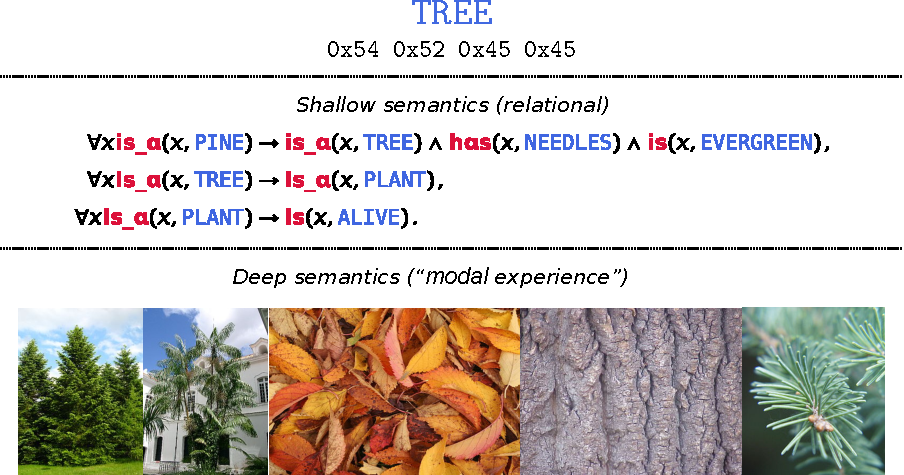
\includegraphics[width=\textwidth]{media/shallow_vs_deep_semantics.pdf}
	\end{frame}

	\begin{frame}{Deep Semantic in Perception: Visual Processing Hierarchy}
		\centering
		\includegraphics[width=0.66\textwidth]{media/htbab_hierarchy.pdf}
		\ImageSources{Eliasmith, \enquote{How to Build a Brain}, 2013, Figure 3.4}
	\end{frame}

	\begin{frame}{Deep Semantic in Perception: Dereferencing}
		\centering
		\vspace{0.5cm}
		\includegraphics[width=0.975\textwidth]{media/htbab_dereference.pdf}\\
		\vspace{0.0575cm}
		\ImageSources{Eliasmith, \enquote{How to Build a Brain}, 2013, Figure 3.7}
	\end{frame}

	\begin{frame}{Perception vs. Action}
		\centering
		\includegraphics[height=7cm]{media/htbab_perceptual_motor.pdf}
	\end{frame}

	\begin{frame}{Nengo SPA Example (I)}
		\centering
		\includegraphics[width=\textwidth]{media/spa_network.pdf}
	\end{frame}

	\begin{frame}{Nengo SPA Example (II)}
		\centering
		\includegraphics[width=\textwidth]{media/nengo_spa_example.pdf}
	\end{frame}

	

	\begin{frame}{Basal Ganglia (BG)}
		\centering
		\includegraphics[height=7.5cm]{media/basal_ganglia.jpg}
	\end{frame}

	\begin{frame}{Clinical Evidence for the Role of the BG in Action Selection}
		\begin{columns}[t]
			\column{0.5\textwidth}
			\begin{block}{\hl{Parkinson's disease}}
				\begin{itemize}			
					\setlength{\itemsep}{0.5cm}
					\item Neurons in the substantia nigra die off
					\item Difficult to trigger actions to start
					\item Usually physical actions
					\item Cognitive effects in later stages
				\end{itemize}
			\end{block}
			\column{0.5\textwidth}
			\begin{block}{\hl{Huntingtons's disease}}
				\begin{itemize}			
					\setlength{\itemsep}{0.5cm}
					\item Neurons in the striatum die off
					\item Actions triggered inappropriately
					\item Small uncontrollable movements
					\item Trouble sequencing cognitive actions					
				\end{itemize}
			\end{block}
		\end{columns}
	\end{frame}

	\begin{frame}{Neurophysiological Evidence for the Role of the BG in Action Selection}
		\begin{multicols}{2}
		\begin{itemize}
			\setlength{\itemsep}{0.25cm}
			\item Role in reinforcement learning
			\item Dopamine levels map onto reward prediction error
		\end{itemize}
		\end{multicols}
		\centering
		\includegraphics[width=0.8\textwidth]{media/dopamine.png}
	\end{frame}

	\begin{frame}{Microcircuitry of the Basal Ganglia}
		\centering
		\includegraphics[width=0.8\textwidth]{media/basal_ganglia2.png}
	\end{frame}

	\begin{frame}{Simplified Model}
		\centering
		\includegraphics[width=0.8\textwidth]{media/gpr3.png}
		\ImageSources{Gurney, Prescott, and Redgrave, \emph{Model of Action Selection in the Basal Ganglia, 2001}}
	\end{frame}

	\begin{frame}{The Cortex-Basal Ganglia-Thalamus loop}
		\centering
		\includegraphics[width=0.8\textwidth]{media/ctx-bg-thal.png}
	\end{frame}

	\videoframe{nengo_hanoi}{sUvHCs5y0o8}

  \begin{frame}{Recency and Primacy Experiment}
		\centering
		\Large
		\hl{Experiment:} Remember this list (presented one at a time)
		\begin{multicols}{2}
%		\begin{enumerate}
%			\centering
%			\setlength{\itemsep}{0.25cm}
%			\item<2,12> robot
%			\item<3,12> teflon
%			\item<4,12> kettlemaking
%			\item<5,12> big-league
%			\item<6,12> troubleshooter
%			\item<7,12> conglomerates
%			\item<8,12> waxberries
%			\item<9,12> electrograph
%			\item<10,12> overjoyous
%			\item<11,12> unquailing
%		\end{enumerate}
		\begin{enumerate}
			\centering
			\setlength{\itemsep}{0.25cm}
			\item robot
			\item teflon
			\item kettlemaking
			\item big-league
			\item troubleshooter
			\item conglomerates
			\item waxberries
			\item electrograph
			\item overjoyous
			\item unquailing
		\end{enumerate}
		\end{multicols}
	\end{frame}

	\begin{frame}{Recency and Primacy Data}
		\centering
		\includegraphics[width=0.6\textwidth]{media/htbab_recall_accuracy_jahnke.pdf}
	\end{frame}

	\begin{frame}{Ordinal Serial Encoding (OSE) Model}
		\centering
		\includegraphics[width=0.9\textwidth]{media/htbab_ose.pdf}
	\end{frame}

	\begin{frame}{Ordinal Serial Encoding (OSE) Model: Experiment}
		\centering
		\includegraphics[width=\textwidth]{media/htbab_ose_experiment.pdf}
	\end{frame}

  \begin{frame}{Spaun -- Semantic Pointer Architecture Unified Network (I)}
		\centering
		\includegraphics[width=0.8\textwidth]{media/eliasmith_2012_spaun_architecture.pdf}
	\end{frame}
	
	\begin{frame}{Spaun -- Semantic Pointer Architecture Unified Network (II)}
		\centering
		\includegraphics[width=0.8\textwidth]{media/eliasmith_2012_spaun_anatomy.pdf}
	\end{frame}


	\backupbegin

	\begin{frame}[noframenumbering]{Image sources}
		\small
		\textbf{Title slide}\\\emph{Librarian (In a library)}, between 1850 and 1866,  Georg Reimer\\ \href{https://commons.wikimedia.org/wiki/File:Reimer_Librarian.jpg}{Wikimedia}.
	\end{frame}

	\backupend
	
\end{document}
